\section{Menu}\label{menu}
\pvelist{ \pve{4.6.5}, \pve{4.6.5}, \pve{4.6.6} }
Via een aparte sectie in de beheeromgeving kunnen de beschikbare menu's worden aangepast. Het menu systeem staat in Drupal los van de inhoud (nodes). Om een pagina in het menu toe te voegen zal eerst de pagina toegevoegd moeten worden en kan daarna het menu-item worden aangemaakt.

Voor \customerdomain  zijn er verschillende menu's in gebruik. Bovenin staat een corporate menu. Deze bevat de links \emph{home}, \emph{over ons}, \emph{pers} en \emph{contact}. De naam van dit menu is \emph{Corporate menu}. Voor de footer zijn de volgende menu's beschikbaar:
\begin{itemize}
\item Footer kolom 1
\item Footer kolom 2
\item Footer kolom 3
\end{itemize}
Elke doelgroep heeft ook een aantal menu's:
\begin{itemize}
\item Doelgroep kolom 1
\item Doelgroep kolom 2
\item Doelgroep kolom 3
\item Doelgroep kolom 4
\item Doelgroep corporate
\end{itemize}
Op de algemene homepage (\texttt{http://\customerdomain /}) zijn de kolom 1 t/m 4 menu's te zien van alle doelgroepen (in een overlay).

Het corporate menu dat rechtsbovenin staat kan per subsite worden aangepast door het bijbehorende menu aan te passen (bijv. \emph{Reizigers corporate}).

Ga hiervoor naar \emph{Structuur} $\rightarrow$ \emph{Menu's} of direct naar \drupalpath{admin/structure/menu}. Klik rechts van het te bewerken menu op \emph{links weergeven} om de links in dat menu te bekijken.

Op deze pagina kan de volgorde van de menu-items bepaald worden via \emph{drag \& drop}. Hiermee kan ook de hi\"{e}rarchie worden aangepast.

\subsubsection{Item toevoegen}\label{menuitemtoevoegen}
Klik op de link \emph{Link toevoegen} bovenaan de pagina om een menu-link toe te voegen. Op de volgende pagina verschijnen de volgende relevante velden:
\begin{itemize}
\item Titel van menulink \\
  Naam waaronder deze pagina in het menu te zien is. Vaak zal dit hetzelfde zijn als de paginatitel.
\item Pad \\
  Het pad van de pagina dat toegevoegd moet worden. Dit kan een volledige URL zijn of een relatief pad. Neem ook het protocol (\texttt{http://}) mee bij het gebruik van een volledige URL. Een relatief pad is zonder domeinnaam en zonder slashes aan het begin en eind.
\item Bovenliggend onderdeel \\
  Dit bepaald de hi\"{e}rarchie.
\item Gewicht \\
  Dit bepaald de positie in het menu. Items met een hoger gewicht komen lager te staan.
\item Afbeelding \\
  Hier kan de afbeelding voor de carrousel worden toegevoegd.
\end{itemize}
Vul de relevante velden in en klik op \emph{Opslaan} om het menu-item aan te maken.

De doelgroep moet niet meegenomen worden in het pad. Bij nodes kan de alias\seeone{alias} worden gebruikt (pad zonder doelgroep) of systeempad ("node/304"). Bij het linken naar een homepage (algemeen of doelgroep) moet de volledige url worden opgegeven (volledige url is wel met doelgroep). Hieronder staan een aantal vooorbeelden:
\begin{itemize}
\item Link naar: \drupalpath{/omwonenden/waarom-wiebelen-treinen} \\
Vul in: "waarom-wiebelen-treinen" of "node/304"
\item Link naar: \drupalpath{/omwonenden} \\
Vul in: "\drupalpath{/omwonenden}"
\item Link naar: http://www.prorail.nl \\
Vul in: "http://www.prorail.nl"
\end{itemize}

\subsubsection{Item bewerken}
Klik in het menu overzicht\seeone{menubeheer} op de link \emph{bewerken} rechts van het menu-item dat aangepast moet worden. Hierna verschijnt eenzelfde formulier als bij het toevoegen van menu-items\seeone{menuitemtoevoegen}.

\subsubsection{Item verwijderen}
Klik in het menu overzicht\seeone{menubeheer} op de link \emph{verwijderen} rechts van het menu-item dat verwijderd moet worden. Deze handeling moet worden bevestigd.

\subsubsection{Footermenu}
\pvelist{ \pve{4.10}, \pve{4.10.1}, \pve{4.10.3}, \pve{4.10.4}, \pve{4.10.6}, \pve{4.10.7} }
Voor het footermenu is er een menu per kolom beschikbaar\seeone{menu}. Per kolom kunnen items worden toegevoegd en bewerkt worden. De volgorde en namen kunnen aangepast worden volgens de beschrijvingen eerder in deze sectie. Alle items die worden toegevoegd aan dit menu worden getoond aan de gebruiker. Het aantal items staat dus niet vast. De eerste link wordt iets los getoond en is visueel de kolomheader.

\subsubsection{Toevoegen van content}
Op de pagina \drupalpath{admin/structure/menu/manage/navigation} kun je de volgorde aanpassen van \drupalpath{node/add}

\subsubsection{Menu-items in meerdere menu's}\label{menumultishizzle}
Het corporate menu en het footer menu is beschikbaar per subsite. Deze kan ook per subsite verschillend zijn. Er is wel een voorziening waarmee wijzigingen in het menu doorgevoerd worden in de menu's van andere subsites. Standaard zal bij het aanmaken van een nieuw item automatisch een kopie van het item worden aangemaakt in de andere menu's. Bij het bewerken van \'{e}\'{e}n van de items zal de wijziging ook automatisch op alle items worden doorgevoerd. Het is mogelijk om dit gedrag voor specifieke menu-items te be\"{i}nvloeden.

Bij het aanmaken of bewerken van een menu-item is er een onderdeel in het formulier met de naam \emph{Subsite menu's}. In dit onderdeel staan vinkhokjes voor alle menu's uit overige subsites. Bij nieuwe items zullen deze standaard aangevinkt zijn. Dat wil zeggen dat een kopie in deze menu's wordt aangemaakt. Wanneer het niet gewenst is dat er een kopie wordt gemaakt dan kan deze optie per menu worden uitgezet.

\begin{center}
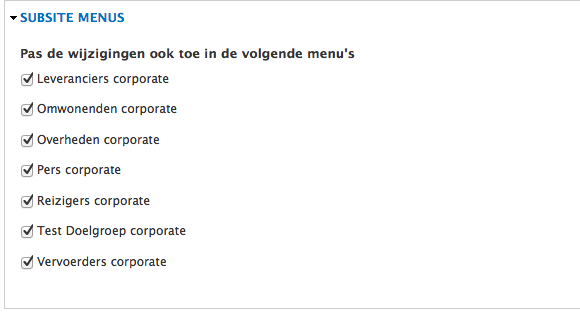
\includegraphics[scale=.7]{img/menukopie.png}
\end{center}

Indien een menu-item wordt bewerkt zullen alle menu's die een kopie bevatten standaard aangevinkt zijn. Wijzigingen worden ook verwerkt in deze menu's. Als een wijziging enkel voor het huidige menu toegepast dient te worden dan moeten de vinkjes dus weggehaald worden. Daarna wijkt dit item af van de items in de overige menu's. Daarmee zal het item niet meer worden gezien als een kopie en worden wijzigingen in andere items dus niet meer toegepast op dit item.

Bij het verwijderen van een item zal deze lijst ook zichtbaar zijn. Standaard zal elke kopie ook worden verwijderd. Indien dit niet gewenst is kunnen ook hier de vinkjes weggehaald worden per menu.

Indien een item wordt bewerkt waarvan geen kopie beschikbaar is in een bepaald menu dan zal dat menu standaard niet zijn aangevinkt op de bewerkpagina. Het is wel mogelijk om deze aan te zetten. In dat geval wordt alsnog een kopie van het menu-item gemaakt in het desbetreffende menu.

\subsubsection{Contactinformatie in vierde menukolom}\label{menumultishizzle}
De teksten zijn per doelgroep instelbaar. Wijzig hiervoor het menu-item in het hoofdmenu:
\drupalpath{/admin/structure/menu/manage/main-menu}

